\chapter{TINJAUAN PUSTAKA}
\label{chap:tinjauanpustaka}

\section{Hasil penelitian/perancangan terdahulu}
\label{sec:HasilTerdahulu}
\begin{enumerate}
  \item \emph{Driver Drowsiness Detection Through HMM based Dynamic Modeling} Eyosias Tadesse, Weihua Sheng and Meiqin Liu (2014)
  
  \parencite{6907440} melakukan penelitian untuk mengetahui kondisi kantuk
  pengemudi dengan menggunakan ekspresi wajah dan model berbasis HMM atau Hidden Markov Model.
  Hasilnya menunjukkan bahwa terdapat perbedaan akurasi dari model yang digunakan. Dimana Deteksi kantuk
  dengan pengenalan ekspresi wajah menunjukkan hasil akurasi yang lebih rendah daripada model HMM.

  \item \emph{Eye State Detection Based on EAR and HOG PSO-Support Vector Machine} Liang CHEN and Wei Zhang (2023)

  \parencite{10270738} melakukan penelitian dengan menggunakan metode Nilai bukaan mata dan 
  dengan HOG PSO-SVM. Penelitian ini bertujuan untuk mendeteksi kondisi kedipan mata dengan 
  menggunakan EAR. Dengan menggunakan model retina wajah,titik titik kunci dari mata dan wajah 
  manusia bisa didapatkan. Algoritma PSO digunakan dan di test pada data set yang dimiliki. Hasil akurasi yang 
  didapatkan adalah dengan nilai 0.98. Dimana waktu yang dibutuhkan untuk memproses gambar dengan 
  metode EAR-HOG-SVM adalah sekitar 3ms.
  
  \item \emph{Research on the Fatigue Detection Method of Operators in Digital Main Control Rooms of Nuclear Power Plants based on Multi-Feature Fusion}
  Guangyu Liu,Jie Liu and Licao Dai (2023)

  \parencite{tan2018research}melakukan penelitian dengan tujuan untuk mendeteksi kantuk pada Operators Ruang Kontrol Pembangkit Listrik 
  tenaga Nuklir. Penelitian ini dilakukan dengan menggunakan PERCLOS atau Percentage Of Eyelid Closure. 
  Metode ini bekerja dengan mendeteksi bukaan mata manusia, kemudian mengklasifikannya dengan data 
  yang telah didapat dari hasil deteksi. Hasil dari penelitian ini menunjukkan hasil yang cukup positif. 
  Nilai akurasi yang didapat mencapai 80.89.
\end{enumerate}

\section{Teori/Konsep Dasar}
\label{sec:DasarTeori}

\subsection{Facial Landmarks}
\label{subsec:FacialLandmarks}


Facial landmarks adalah titik-titik kunci pada wajah manusia 
yang digunakan untuk mengidentifikasi dan menganalisis 
fitur-fitur wajah secara spesifik, seperti mata, hidung, 
mulut, dan kontur wajah. Teknik deteksi facial landmarks 
merupakan komponen penting dalam berbagai aplikasi pengolahan 
citra dan visi komputer, termasuk dalam sistem pengenalan wajah, 
filter wajah interaktif pada aplikasi kamera, serta untuk 
analisis ekspresi wajah. Dengan menggunakan algoritma machine 
learning dan deep learning, seperti Convolutional Neural 
Networks (CNN), sistem dapat dilatih untuk secara akurat 
mendeteksi dan melacak landmark wajah dalam gambar atau video 
secara real-time. Deteksi ini umumnya melibatkan langkah-langkah 
seperti deteksi wajah terlebih dahulu untuk menentukan region of 
interest (ROI), diikuti oleh identifikasi dan pemetaan 
titik-titik landmark spesifik\parencite{johnston2018review}. Hasil dari proses ini memungkinkan 
aplikasi untuk melakukan tugas-tugas seperti penyesuaian fitur 
wajah, animasi wajah, atau deteksi kantuk dengan menggunakan titik pada 
wajah manusia.

Facial landmark juga  dapat digunakan sebagai metodee untuk mendeteksi 
keadaan ekspresi seseorang seperti penelitian yang dilakukan oleh Gopalan,
Bellamkonda, and Chaitanya\parencite{gopalan2018facial}. Penelitian yang dilakukan mengimplementasikan 
konsep titik titik pada wajah dan kemudian dilakukan deep learning dengan menggunakan 
metode CNN (Convolutional Neural Networks). Dengan beberapa dataset yang dimiliki,
setiap dataset diberikan landmark pada wajah objek yang kemudian diolah menjadi sebuah sistem untuk 
mendeteksi ekspresi dari objek tersebut.


\begin{figure} [H] \centering
  % Nama dari file gambar yang diinputkan
  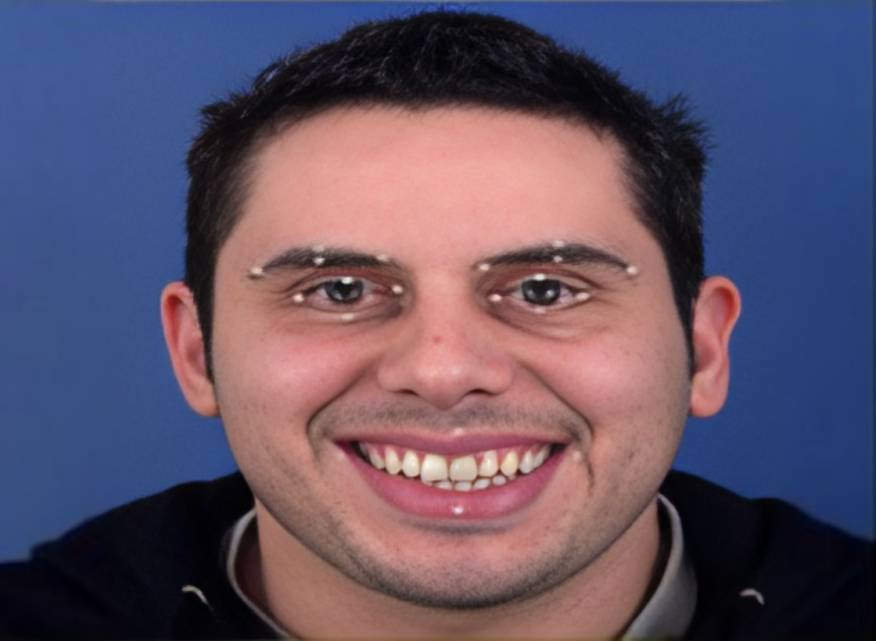
\includegraphics[scale=0.2]{gambar/2_2_1.png}
  % Keterangan gambar yang diinputkan
  \caption{\emph{Facial Landmarks} pada wajah objek}
  % Label referensi dari gambar yang diinputkan
  \label{fig:FacialLandmarks}
\end{figure}



\subsection{Deep learning}
\label{subsec:DeepLearning}

Deep learning merupakan cabang dari pembelajaran mesin yang 
menggunakan jaringan neural tiruan dengan banyak lapisan untuk 
memodelkan abstraksi data tingkat tinggi. Cara kerjanya 
melibatkan pemrosesan data melalui lapisan ini, dimana setiap 
lapisan secara otomatis dan secara progresif mempelajari 
fitur-fitur semakin kompleks dari data\parencite{akbulut2017deep}. Berbeda dengan 
pembelajaran mesin tradisional, deep learning dapat secara 
otomatis mengekstrak fitur penting tanpa memerlukan intervensi 
manual, memungkinkan model untuk melakukan tugas yang lebih 
kompleks dengan akurasi yang lebih tinggi. Keunggulan utama dari deep 
learning terletak pada kemampuannya untuk mengolah volume data 
yang sangat besar dan kompleks, memungkinkannya mengidentifikasi 
pola dan hubungan yang tidak dapat ditemukan oleh metode 
pembelajaran mesin konvensional. Hal ini membuat deep learning 
sangat efektif dalam aplikasi yang memerlukan analisis mendalam 
dari data visual, auditif, dan teks, memberikan dorongan 
signifikan dalam kemajuan teknologi pengenalan suara, visi 
komputer, dan pemrosesan bahasa alami.


\subsection{Percentage Of Eyelid Closure \emph{(PERCLOS)}}
PERCLOS atau biasa disebut Percentage of Eyelid Closure adalah salah 
satu metode yang digunakan untuk mendeteksi kantuk.
PERCLOS merupakan metrik yang digunakan untuk mengukur kantuk 
atau kelelahan pengemudi. Metode ini bekerja dengan cara 
menghitung persentase waktu dalam interval tertentu dimana dilakukan 
perhitungan bukaan kelopak mata seseorang tertutup sebagian atau 
seluruhnya di atas pupil. PERCLOS berfungsi sebagai indikator 
objektif untuk mengukur tingkat kantuk, berdasarkan frekuensi dan 
durasi penutupan mata meningkat seiring dengan kelelahan. 
PERCLOS efektif menunjukkan tingkat kelelahan pengemudi dan 
dianggap metode terbaik untuk mengukur kelelahan. Metode ini 
menghitung persentase waktu mata tertutup setidaknya 70 
atau 80 persen dari durasi total, yang umumnya adalah 30 
detik atau 1 menit. Guangyu,Jie,Licao melakukan penelitian dengan 
mengukur PERCLOS dan menghitung persentase frame dengan persentase mata tertutup 80 persen dalam video selama 30 detik 
dibagi dengan total frame selama 30 detik tersebut\parencite{Liu2023}. Atau dapat ditulis

\begin{equation}
  P80 = \frac{Frames with eyes closed to 80\% }{Total Frames of 30s video}
\end{equation}

(Liying,Haoxiang, 2008) menyatakan bahwa Tingkat pembukaan mata 
dapat dicirikan oleh bentuk pupil. Berdasarkan pengamatan bahwa 
saat mata tertutup, pupil mulai terhalang oleh kelopak mata dan 
bentuknya menjadi lebih elips. Oleh karena itu, mereka dapat 
menggunakan rasio sumbu elips pupil untuk menggambarkan tingkat 
pembukaan mata \parencite{lang2008study}. Untuk mendapatkan pengukuran yang lebih kuat 
untuk kedua parameter ini, dilakukan perhitungan rata-rata runtime 
(time tracking). Berdasarkan nilai rata-rata yang didapatkan, 
Liying,dkk dapat menganalisis keadaan waspada pengemudi. Mereka menghitung
2 parameter yang digunakan (rumus 2.1).

\begin{figure} [H] \centering
  % Nama dari file gambar yang diinputkan
  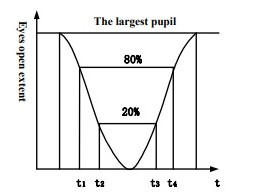
\includegraphics[scale=1]{gambar/2_2_2.jpg}
  % Keterangan gambar yang diinputkan
  \caption{Prinsip PERCLOS}
  % Label referensi dari gambar yang diinputkan
  \label{fig:PERCLOS}
\end{figure}

\subsection{Mouth Aspect Ratio (\emph{MAR})}
\label{subsec:MAR}

MAR atau Rasio Aspek Mulut adalah metrik analisis wajah yang 
digunakan untuk mendeteksi gerakan mulut yang berkaitan dengan 
berbagai kondisi, seperti berbicara, menguap, atau ekspresi emosi. 
Fungsinya adalah sebagai indikator kondisi ini dengan 
memperhitungkan kondisi geometris mulut seseorang pada waktu 
tertentu. Perhitungan MAR melibatkan analisis titik-titik 
tertentu di sekitar mulut dan menghitung rasio berdasarkan jarak 
antara titik-titik tersebut. Rasio ini kemudian dapat dipantau 
dari waktu ke waktu untuk mengamati perubahan yang mungkin sesuai 
dengan perilaku atau ekspresi tertentu. Pada deteksi kantuk,MAR (Mouth Aspect Ratio) dapat mengklasifikasikan kondisi kantuk pengemudi dengan mengukur perubahan geometri mulut berdasarkan titik-titik yang telah ditentukan pada model wajah. Titik-titik ini, yang mengelilingi bibir, digunakan untuk menghitung rasio yang mencerminkan pembukaan mulut. Ketika pengemudi mulai mengantuk, frekuensi dan durasi menguap meningkat, yang tercermin dalam nilai MAR yang lebih tinggi. Dengan memantau nilai ini, sistem dapat secara otomatis mendeteksi tanda-tanda awal kelelahan dan mengeluarkan peringatan kepada pengemudi.

\begin{figure} [H] \centering
  % Nama dari file gambar yang diinputkan
  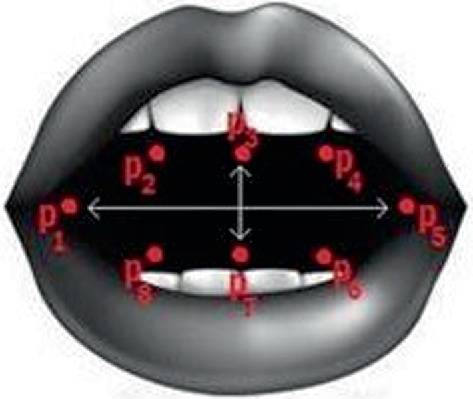
\includegraphics[scale=0.3]{gambar/2_2_3.png}
  % Keterangan gambar yang diinputkan
  \caption{MAR point}
  % Label referensi dari gambar yang diinputkan
  \label{fig:MAR}
\end{figure}


Pada gambar 2.3 terdapat sebanyak 8 titik yang saling berhubungan. titik-titik tersebut nantinya akan digunakan sebagai acuan agar dilakukan perhitungan. Hasil perhitungan ini disebut sebagai hasil lokalisasi kemudian menghasilkan nilai MAR. Nilai MAR dapat ditentukan dengan rumus sebagai berikut. Dimana |p2-p8| adalah nilai hasil perhitungan Jarak Euclidean antara koordinat titik-titik fitur pada wajah, dan delapan titik fitur kunci yang berkorespondensi dengan variabel dalam rumus sebagaimana ditampilkan pada gambar 2.3. Jarak Euclidean ini dihitung dengan mengambil akar kuadrat dari perbedaan kuadrat koordinat horizontal dan vertikal dari dua titik fitur tersebut\parencite{chandiwala2021driver}.

\begin{equation}
MAR = \frac{|{p2} - {p8}| + |{p3} - {p7}| + |{p4} - {p6}|}{3|{p1} - {p5}|}
\end{equation}


\subsection{Skala Kantuk Karolinska}
\label{subsec:KSS}
\newcommand{\w}{}
\newcommand{\G}{\cellcolor{gray}}
\begin{table}[h!]
  \centering
  \caption{Skala Kantuk Karolinska}
  \begin{tabular}{|c|l|}
    \hline
    Skala \G & Penjelasan \G  \\
    \hline
    1 & Amat sangat terjaga \\
    2 & Sangat terjaga \\
    3 & Terjaga \\
    4 & Cukup terjaga \\
    5 & Antara terjaga dan mengantuk \\
    6 & Muncul mengantuk \\
    7 & Mengantuk namun tidak sulit untuk terjaga/kantuk ringan \\
    8 & Sangat mengantuk, sulit terjaga \\
    9 & Amat sangat mengantuk, cenderung tidak sadar \\
    \hline
  \end{tabular}
  \label{tab:SkalaKSS}
\end{table}


Skala Kantuk Karolinska, yang dikenal juga dengan Karolinska Sleepiness Scale (KSS), adalah skala yang digunakan untuk mengukur kantuk secara subjektif. Skala ini berkisar dari 1 hingga 9, dengan 1 mengindikasikan tingkat kesegaran tinggi dan 9 menunjukkan kesulitan yang sangat besar untuk tetap terjaga. Skala Kantuk Karolinska (KSS) dapat digunakan sebagai alat pengklasifikasi kantuk dengan beberapa cara. Pada beberapa penelitian yang telah dilakukan, KSS digunakan sebagai pengklasifikasi kantuk. Dengan metode skala kantuk karolinska,terlihat bahwa klasifikasi kantuk yang dilakukan memiliki hasil akurasi yang tinggi dimana artinya KSS terbukti valid dijadikan sebagai acuan skala klasifikasi kantuk.

\subsection{Support Vector Machine \emph{(SVM)}}
\label{subsec:SVM}

Dalam lingkup Deep learning atau tepatnya supervised learning, Support Vector Machine (SVM) merupakan metode klasifikasi dan regresi yang efektif. SVM beroperasi dengan mengembangkan konsep hyperplane yang optimal, yang secara matematis didefinisikan sebagai batas pemisah yang paling efisien antara kelas-kelas data. Algoritma ini melibatkan identifikasi margin terlebar yang memungkinkan pemisahan kelas dengan paling jelas, yang bertujuan untuk meningkatkan akurasi prediksi model pada data baru. Dalam ruang dua dimensi, hyperplane ini dapat berupa garis lurus, tetapi dalam ruang tiga dimensi atau lebih, ia menjadi bidang pemisahan multidimensi. Kemampuan SVM untuk mengadaptasi diri dengan masalah linear dan non-linear menjadikannya pilihan yang kuat dalam berbagai aplikasi pembelajaran mesin, dari pengenalan gambar hingga pemodelan prediktif dalam keuangan.  

\begin{figure} [H] \centering
  % Nama dari file gambar yang diinputkan
  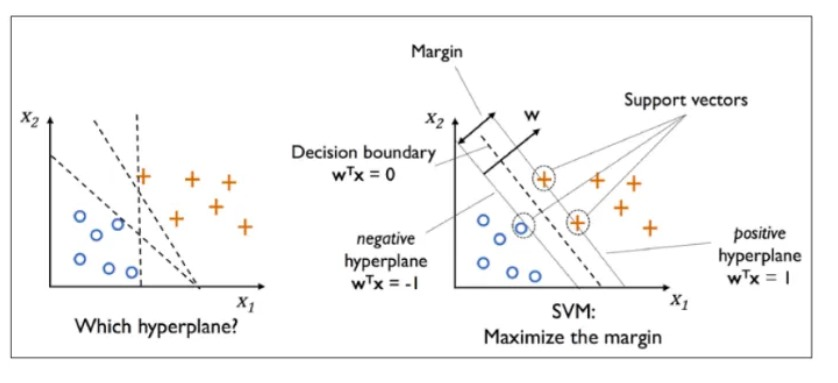
\includegraphics[scale=0.7]{gambar/2_2_6.jpg}
  % Keterangan gambar yang diinputkan
  \caption{Hyperplane yang memisahkan kelas positif dan negatif}
  % Label referensi dari gambar yang diinputkan
  \label{fig:SVM}
\end{figure}

Pada gambar 2.4, dapat dilihat bahwa ada perbedaan jarak antara hyperplane dengan kedua kelas baik itu kelas positif atau negatif dimana pada gambar tersebut kelas negatif bertanda bulat. Dengan SVM, objek terdekat dengan hyperplane dikenali dengan nama Support Vector. Objek tersebut baik itu dari kelas negatif atau positif dapat dikatakan sulit untuk diklasifikasikan. Hal tersebut terjadi karena data kelas tersebut sangat berdekatan dengan data kelas lain sehingga menyebabkan hampir terjadinya overleap\parencite{tan2018research}. Oleh karena itu,dengan menggunakan SVM,kondisi ini dapat dimimalisir dimana hasil dari perhitungan akan memisahkan dan menentukan kelas dari data yang terkena overleap tersebut.


\subsection{SMOTE}
\label{subsec:SMOTE}
SMOTE (Synthetic Minority Over-sampling Technique) adalah metode yang digunakan dalam pengolahan data untuk mengatasi masalah ketidakseimbangan kelas. Teknik ini menghasilkan sampel data sintetis untuk kelas minoritas dengan cara interpolasi antara sampel minoritas yang ada. Hal ini membantu dalam memperbaiki keseimbangan antara kelas minoritas dan mayoritas, dimana hal tersebut merupakan hal yang penting dalam model pembelajaran mesin untuk meningkatkan kinerja dan hasil yang lebih akurat dalam prediksi.


\begin{figure} [H] \centering
  % Nama dari file gambar yang diinputkan
  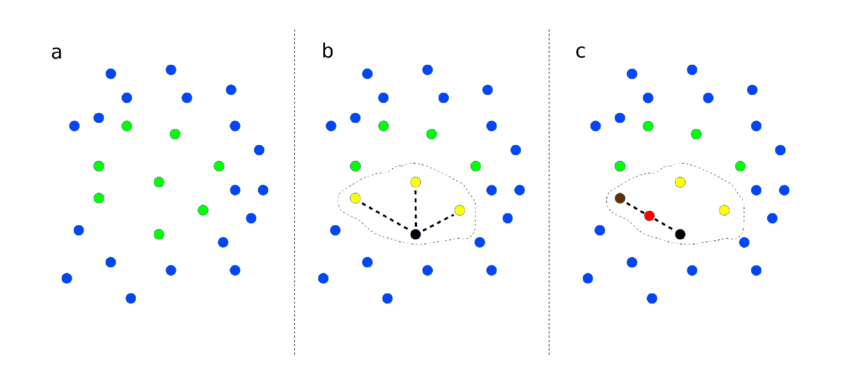
\includegraphics[scale=0.5]{gambar/2_2_5.png}
  % Keterangan gambar yang diinputkan
  \caption{Ilustrasi Visual SMOTE}
  % Label referensi dari gambar yang diinputkan
  \label{fig:SMOTE}
\end{figure}

Gambar 2.4 Merepresentasikan grafis algoritma SMOTE,dimulai dengan sample set positif (titik berwarna hijau),dan sample set negatif (titik berwarna biru). Algoritma ini kemudian memilih sebuah sample positif (titik berwarna hitam) dan kNN diantara titik positif (dengan warna kuning dengan k=3), kemudian akhirnya,salah satu dari kNN secara acak terpilih yang mana kemudian titik positif sintetis baru tercipta dengan secara acak menghasilkan sebuah model baru sepanjang garis lurus yang terhubung dengan titik hitam dan coklat\parencite{schubach2017imbalance}.
